\section{Материалы и методы}
Общая схема эксперимента приведелена на рисунке \ref{scheme}.

\begin{figure}[h]
    \begin{center}
        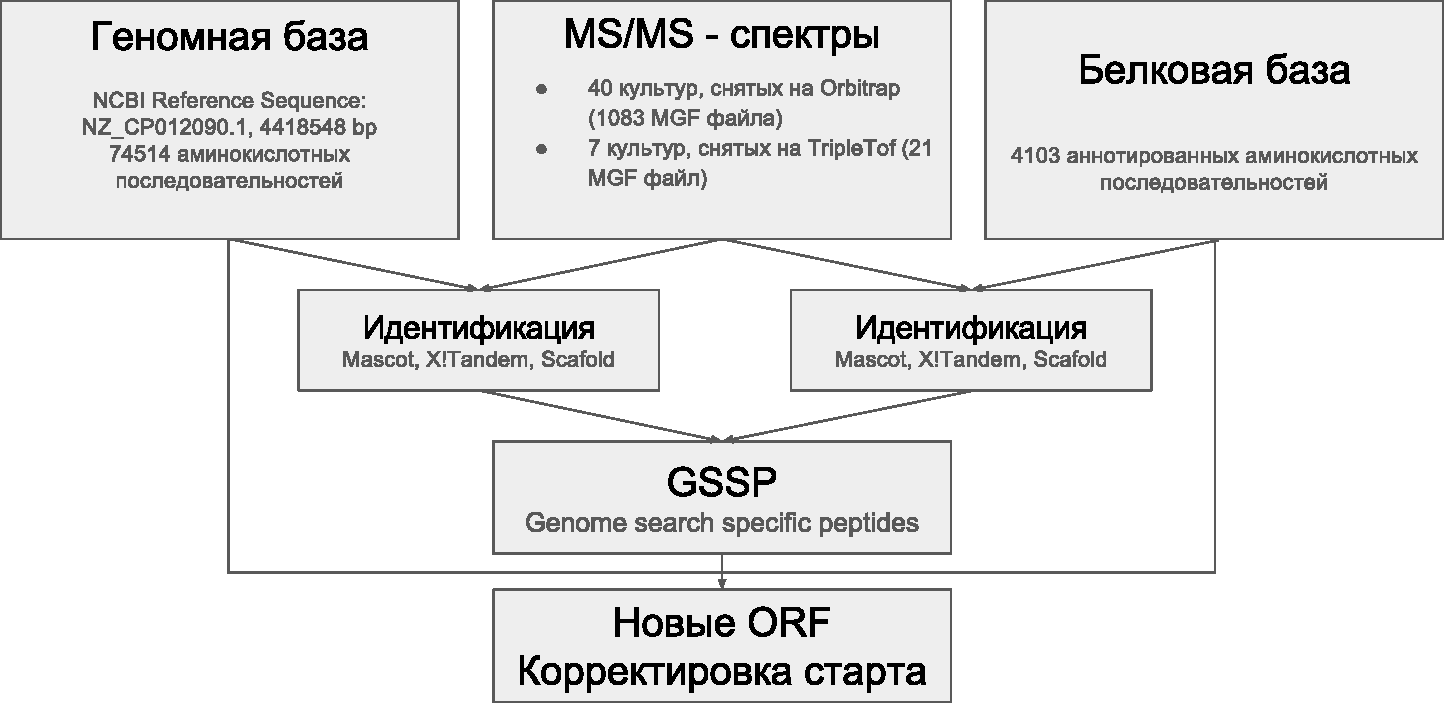
\includegraphics[width=1.\linewidth]{scheme.pdf}
    \end{center}
\caption[foo bar]{Схема анализа масс-спектрометрических данных. Можно выделить следующие ключевые шаги:
  \begin{enumerate*}%[label=\textit{\alph*)}]
    \item идентификация против белковой базы
    \item идентификация против геномной базы
    \item нахождение GSSP
    \item интерпретация GSSP
  \end{enumerate*}.}\label{scheme}
\end{figure}

\subsection{Получение бактерий}
Бактерии были выделены из мокроты, больных туберкулёзом пациентов. 

\subsection{Проведение масс-спектрометрического эксперимента}
Для протеогеномного анализа использовались масс-спектры белковых клеточных лизатов для \ti{M. tuberculosis}, полученных с прибора \fl{AB SCIEX TripleTOF 5600} в лаборатории протеомного анализа НИИ ФХМ и \fl{ThermoFisher Q Exactive Hybrid Quadrupole-Orbitrap} в ИБМХ. 

\subsection{Контроль качества}
Для всех масс-спектров был проведен контроль качества масс-спектров с использованием программного решения реализованного в лаборатории биоинформатики НИИ ФХМ. В ходе контроля качества были проверены следующие факторы: качество трипсинолиза, распределение зарядов родительских ионов, ошибка измерения m/z для родительских и дочерних ионов, распределение идентифицированных пептидов по времени удерживания пептидов в хроматографической колонке.

\subsection{Создание поисковых баз}
В работе использовалось 2 типа баз: белковая и геномная. Белковая база - аннотированные последовательности, для данного штамма. Геноманя - база, полученная в результате транслирования генома в шести рамках.
Белковые базы для \ti{M.tuberculosis W-148} и \ti{M.tuberculosis H37Rv} были составлены из аннотированных белков штаммов (\ti{W-148}: \fl{NCBI Reference Sequence: NZ\_CP012090.1}, версия от 11 марта 2017 года, 4103 аминокислотных последовательности, 137 псевдогена; \ti{H37Rv}: \fl{NCBI Reference Sequence: NC\_000962.3}, версия от 2 августа 2016 года, 3932 аминокислотных последовательности).
Геномные базы были получены в результате 6 рамочного транслирования от стоп- до стоп-каднона геномов штаммов \ti{M.tuberculosis W-148} и \ti{M.tuberculosis H37Rv}, используя программу \fl{Artemis} версия 16.0.0 \cite{rutherford2000artemis}. При транслировании использовалась 11 трансляционная таблица \fl{NCBI}. Минимальная длинна рамки была установлена в 100 нуклеиновых кислот.
К каждой базе были добавлены последовательности 26 контаминантных белков (кератины, альбумины, трипин) и decoy-последовательности, полученные в результате прочтения аминокислотных последовательностей с конца, за исключением стартового метеонина. 

\subsection{Идентификация пептидов и белков}
Данные полученные в результате LC-MS/MS эксперимента (Raw формат) были сконвертированы в пик-лист (MGF формат), используя \fl{ProteoWizard msconvert} \cite{chambers2012cross}. Идентификация проходила против двух белковых и двух геномных баз с использованием \fl{Mascot Search Engine version 2.5.1} \cite{cottrell1999probability} и \fl{X!Tandem version 3.4.3} \cite{fenyo2003method}. Результаты идентификации двух программ были объеденины в \fl{Scaffold version 4.2.1}. 

Параметры поиска \fl{Mascot} были следующими: триптические пептиды, не более одного пропущенного сайта трипсинолиза, ошибка массы прекурсера 20 ppm, ошибка массы фрагментов 0.04 Да, заряды прекурсера 2+, 3+, 4+. \fl{Oxidation(M)} была устанолвена как возможнная модификация пептидов, \fl{Carbamidomethylation(C)} как фиксированная. 

Параметры \fl{X!Tandem} были следующими: триптические пептиды, не более одного пропущенного сайта трипсинолиза, ошибка массы прекурсера 20 ppm, ошибка массы фрагментов 50 ppm, проверка не моноизотопных масс, \fl{Carbamidomethylation(C)} - фиксированная модификация, \fl{Oxidation(M)} возможная модификация.

Результаты работы поисковых машин были объединины в \fl{Scaffold} с параметрами: 1:1 \fl{forward/decoy ratio}, \fl{LFDR scoring}, стандартные белковые группы, не проводить GO-аннотацию. Белковый и пептидный FDR был установлен на уровне 1\%, 1 и более пептидов на белок. Результаты были экспортированны в виде листа идентифицированных пептидов.

\subsection{Протеогеномика \ti{W-148}}
Координаты аннотированных генов были пересечены с учетом стренда и фрейма с координатами ORF, полученными в результате шестирамочного транслирования.
Для поиска GSSP из результатов поиска против геномной базы \ti{W-148} были исключены пептиды, идентифицированные против белковой базы \ti{W-148}. Так же были исключены пептиды идентифицируемые против геномной базы и предсталвенные в аннотации, и пептиды, идентифицируемые только в одной культуре. Для дальнейшего анализа были выбраны ORF, в которых произошло одно из следующих событий:
\begin{inparaenum}
    \item идентифицированно два и более уникальных GSSP
    \item идентифицированн GSSP и присутствует аннотированный ген
    \item идентифицированн GSSP и есть пересечение по координатам с псевдогеном в пределах стренда
\end{inparaenum}.

\subsubsection{Валидация результатов идентификации}
Для каждого GSSP была проведена проверка времени выхода и ошибки масс при идентификации; потенциальной остаточной контаминации на приборе; ошибки интерпретации модифицированной акминокислоты, как другой немодифицированной.

Проверка ошибки идентификации масс проходила на уровне PSM. В каждом ране, для каждого PSM, соответсвующему GSSP, находилась среднее значение и стандартное отклонение ошибки идентификации всех PSM в диапазоне +/- 5 минут от времени выхода данного PSM. Из дальнейшенго анализа исключались все PSM, ошибка идентификации масс которых отличалась более чем на 3 стандартных отклоения от средей ошибки в установленном временом интервале. В каждом ране были отфильтрованны 5\% самых ранних и поздних по времи выхода PSM.

Был проведен поиск точного и с учетом одной возможной замены вхождения GSSP в другие белки, предсталвенные в базе \fl{NCBInr}.  


\subsubsection{Идентификация новых белков}
Рассматривались ORF, в которых было идентифицированно два и более уникальных GSSP-пептида и в которых не содержится аннотиванный ген. Для проверки потенциала кодирующей способности рамки, был проведён blastp против базы nr. 

\subsubsection{Уточнение N-концов}
Рассматривались ORF, в которых было идентифицированно два и более уникальных GSSP-пептида и в которых содержится аннотиванный ген. Новые рамки сравнивались с аналогичными генами в \ti{H37Rv}.

%  \subsection{Сравнение идентификаций против \ti{W-148} и \ti{H37Rv}}
%  \subsubsection{Поиск новый генов}
%  \subsubsection{Уточнение N-концов}

\subsection{Визуалиция данных}
Для визуализации данных использовался \fl{Gbrowse}. Были выделены следующие глифы: 
\begin{inparaenum}
    \item аннотированные гены
    \item идентифицированные пептиды
    \item псевдогены
    \item ORF с новыми генами
    \item ORF с пептидами, идентифицируемые перед аннотированным стартом
    \item GSSP-пептиды.
\end{inparaenum} Результаты идентификации были обработаны и экспортированны в gff3 формате.


\newpage

%\subsection{Тест шрифта с бакалавром}
%пути внутри клетки. Подобная информация может быть применена в медицинских целях. 

%Для количественного анализа белка можно использовать различные методы, например Гель-электрофорез, капиллярный электрофорез, жидкостную хроматографию, различные оптические и спектрографические измерения, центрифугирование, масс-спектрометрию и множество других. Наиболее эффективным методом для количественного анализа сложной смести белков является комбинация жидкостной хроматографии (или высоко эффективной жидкостной хроматографии) с масс-спектрометрией (или тандемной масс-спектрометрии). Это позволяет устанавливать количественный состав смеси не только при помощи сложного процесса меченья белков, но и посредством безметочного анализа состава смеси, как относительного, так и абсолютного. 

%Melioribacter resous - недавно открытая, умеренно теплолюбивая, факультативно анаэробная, хемоорганотрофическая бактерия . Её штамм P3M-2 был получен из микробной плёнки, развивающийся в жёлобе, покрытом древесной корой, находящимся под потоком горячей воды (температура 46 o C), выходящей из поисково-разведочной нефтяной скважины глубиной в 2775 метров, находящейся недалеко от Томска в России. Метаболически универсальная бактерия, способная расти за счёт питания сахарами или пептидами, за счёт аэробного дыхания, нитратов или Fe(III). Недавний анализ генома выделил ключевые элементы цепи переноса электронов, позволяющий понять способность бактерии адаптироваться к изменяющимся условиям окружающей среды, за счёт комбинации окисления различных доноров электронов при аэробном дыхании или сокращения акцепторов электронов 5 .
